\begin{frame}{Effects of Sublimation near Mamers Valles}

\begin{figure}
\centering

\begin{subfigure}{0.48\textwidth}
    \centering
    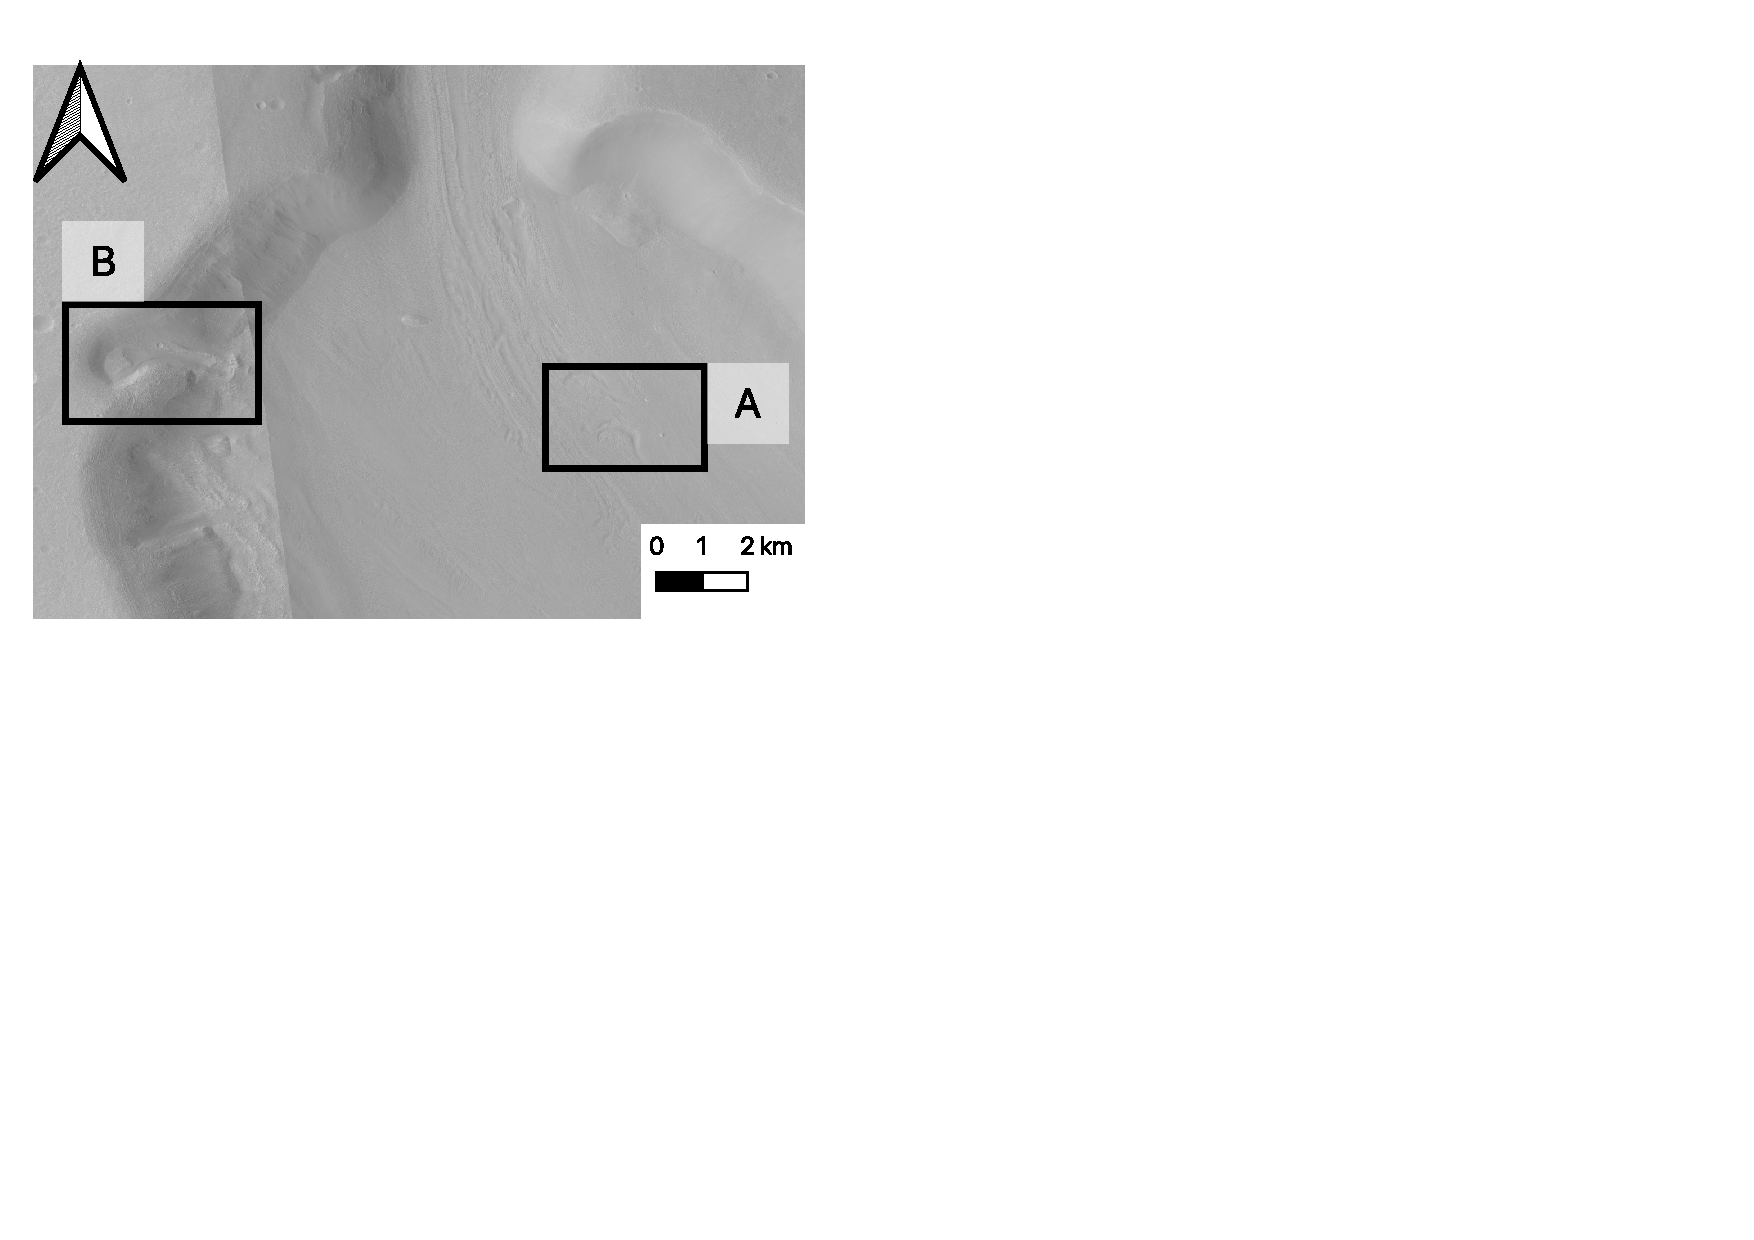
\includegraphics[
        width=\linewidth,
        height=0.65\textheight,
        keepaspectratio
    ]{Figures/CTX/IceActivity_Img.pdf}
    \label{fig:IceActivity_a}
\end{subfigure}
\hfill
\begin{subfigure}{0.48\textwidth}
    \centering
    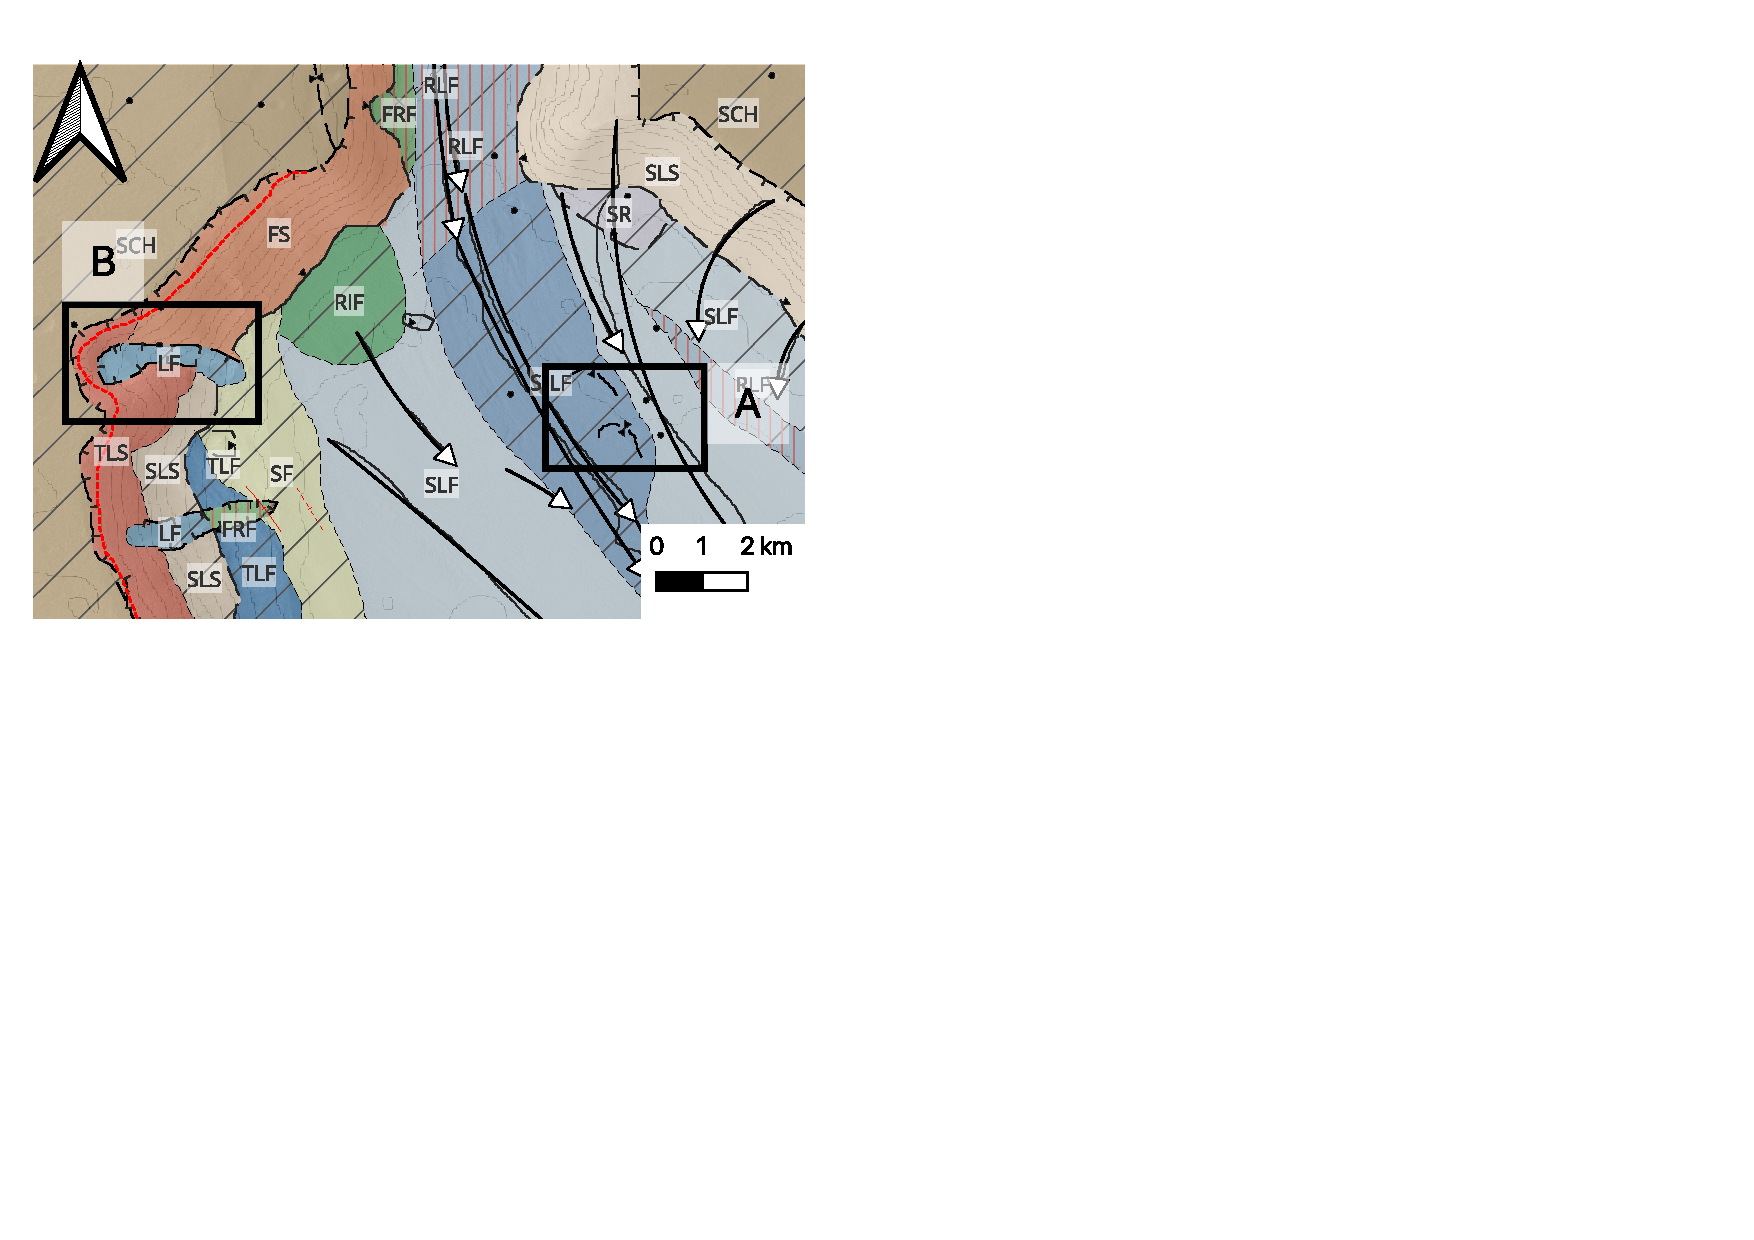
\includegraphics[
        width=\linewidth,
        height=0.65\textheight,
        keepaspectratio
    ]{Figures/CTX/IceActivity_Map.pdf}
    \label{fig:IceActivity_b}
\end{subfigure}

\caption{An overview at the boundary of Ismenius Cavus and the LVF of Mamers Valles (centred at $34.61421^{\circ}$N, $16.92877^{\circ}$E).}
\label{fig:IceActivity}

\end{figure}

\end{frame}

\begin{frame}{Effects of Sublimation near Mamers Valles}
    \begin{figure}
        \centering
        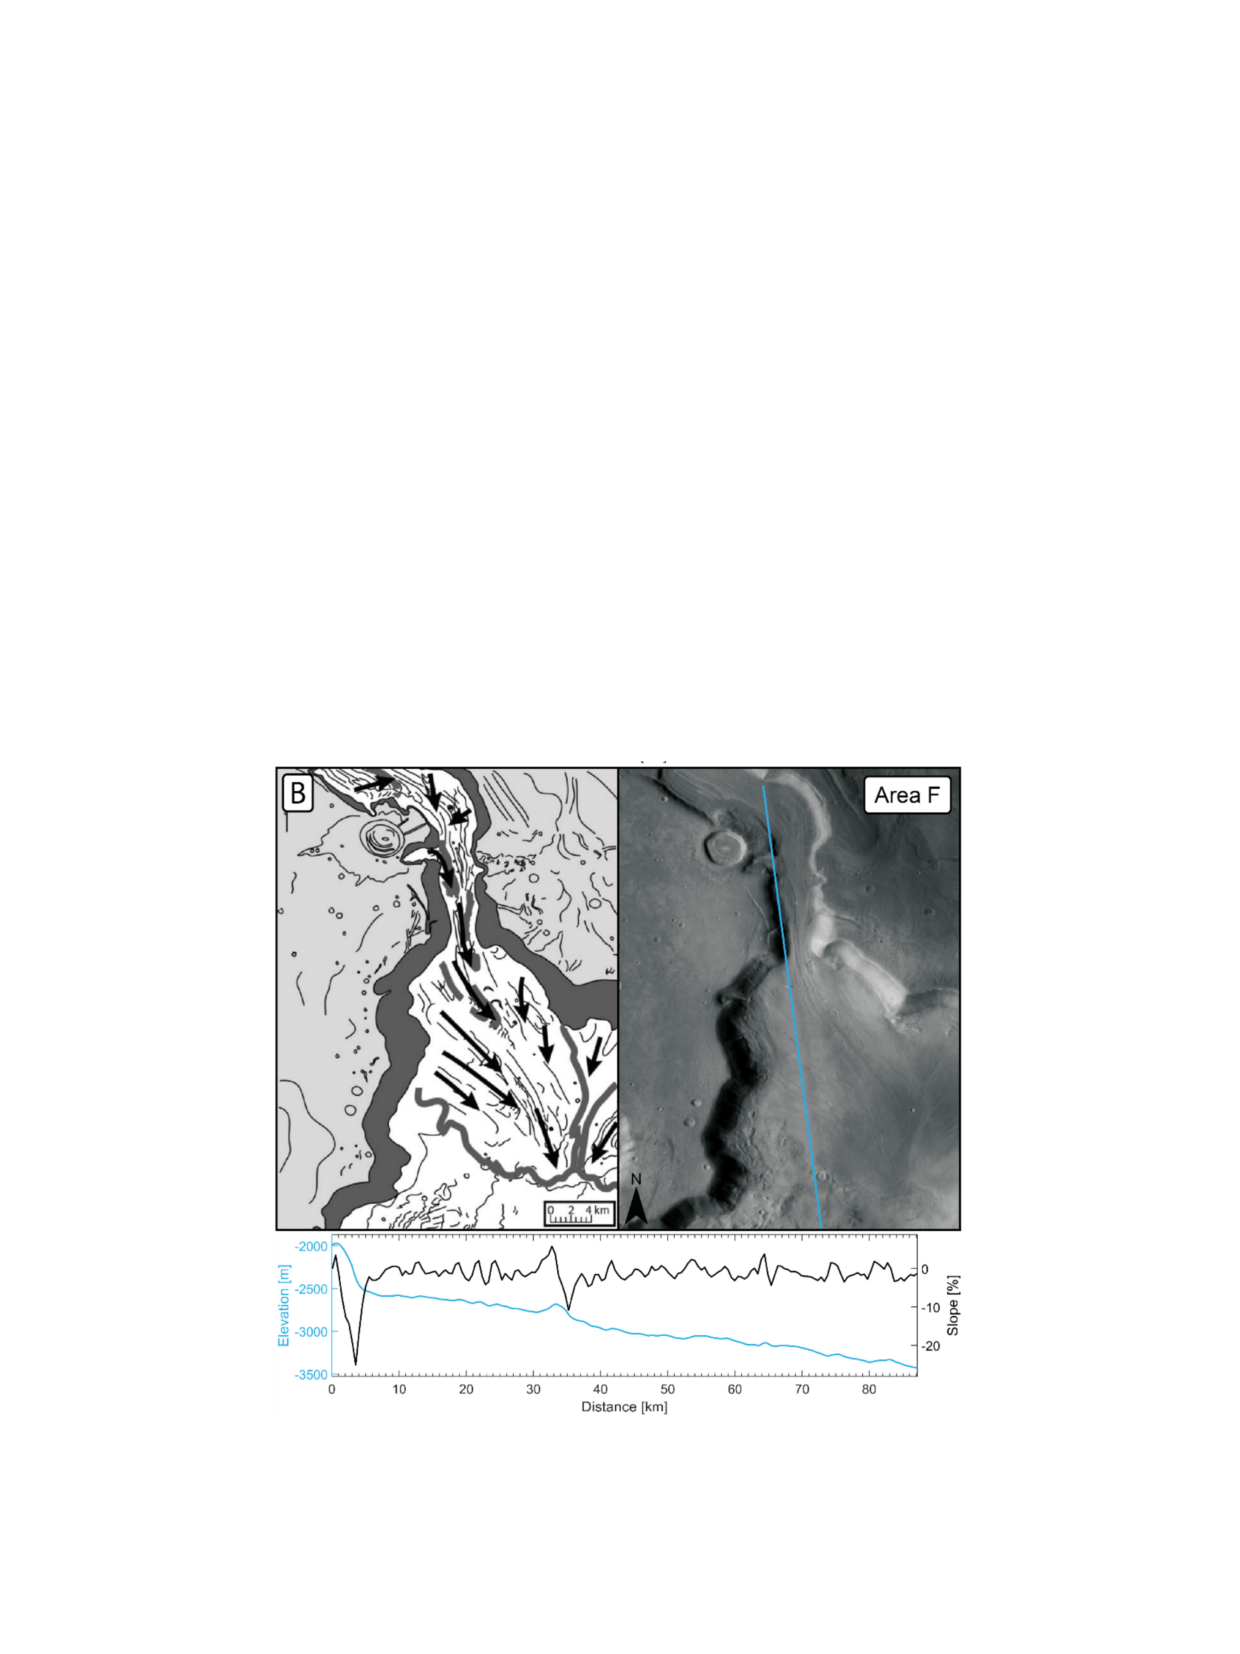
\includegraphics[
        width=\linewidth,
        height=0.65\textheight,
        keepaspectratio]
        {Figures/Diagrams/Wueller25_Fig4}
    \caption{Annotated CTX image data, showing the flow of LVF from Mamers Valles into Ismenius Cavus and the corresponding HRSC-MOLA topographic profile (Figure from \cite{Wueller25}).}
    \end{figure}
\end{frame}
